\documentclass{article}

\usepackage{amsmath}
\usepackage{amsfonts}
\usepackage{mathtools}
\usepackage{graphicx}

\begin{document}
{\centering \LARGE Method \#RDS-4\\}
\section{Shape Representation}

\subsection{Objects Shape Representation}

The method approximates objects' shapes surrounding the robot as a union of circles (see Fig. \ref{fig:shapes}). The set $ C^O $ contains these circles to represent all the surrounding objects' aggregate shape and is defined as
\begin{align*}
C^O = \left\{ c_1^O, ... , c_N^O \right\} ,
\end{align*}
where a given circle $ c_i^O $ represents a part of an object and is characterized by its radius $ r_i^O $ and its center point $ P_i^O $.

%position $ \vec p_i^{\,O} $ with respect to a fixed global coordinate origin.

\subsection{Robot Shape Representation}

The robot's shape is represented by a capsule, which is defined as the shape which results from sweeping a circle along a line segment (see Fig. \ref{fig:shapes}). It is therefore characterized by the swept circle's radius $ r^R $ and the line segment endpoints.
%'s positions with respect to the fixed global coordinate origin. 

The set $ C^R $ is then defined in respect of the set $ C^O $ such that it contains for each object circle $ c_i^O $ the corresponding circle which lies inside the capsule, has radius $ r^R $ and is closest to $ c_i^O  $. This set is denoted as
\begin{align*}
C^R = \left\{ c_1^R, ... , c_N^R \right\} ,
\end{align*}
where each robot circle $ c_i^R $ is characterized by its radius $ r^R $ and its center point $ P_i^R $.
%'s position $ \vec p_i^{\,R} $ with respect to the fixed global coordinate origin.
Note that their center points lie on the capsule's line segment. Fig. \ref{fig:shapes} illustrates these geometric objects' definitions and how they relate to each other.

\begin{figure}
	\begin{center}
		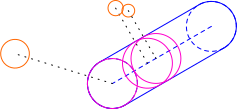
\includegraphics[width=0.8\textwidth]{geometric_objects_relations.pdf}
	\end{center}
	\caption{Showing an example of the robot's capsule (solid blue boundary), some objects' circles (orange) and the corresponding robot circles (magenta).}\label{fig:shapes}
\end{figure}

\section{Robot Kinematics}\label{sec:kinematics}

The method assumes that the robot is a vehicle with two actuated wheels that do not slip and that rotate around the same axle (and with additional caster wheels to stabilize it). The robot's local frame is defined as the Cartesian coordinate frame whose x-axis coincides with the main wheels' axle and whose y-coordinate points forward and intercepts the axle at its midpoint (see Fig. \ref{fig:kinematics}). In the remainder, we always assume the robot's local Cartesian frame to provide the underlying basis vectors when giving explicit coordinates for a vector.

We denote the axle midpoint velocity's $ y $-coordinate by $ v $ and the vehicle's angular velocity by $ \omega $, and we consider the pair $ (v,\omega) $ as the velocity command for the robot. Let the coordinates $ v_x^P, v_y^P $ describe the (global) velocity of a point $ P $ on the robot (expressed in the local frame). The point's Jacobian $ J_P $ is defined as the matrix which maps any velocity command on the resulting point velocity according to $ {[v_x^P, v_y^P]}^T =  J_P {[v, \omega]}^T $. The inverse $ J_P^{-1} $ exists for any point $ P $ which does not lie on the wheel axle. Thus, the velocity of any point $ P' $ is determined by the velocity of any other point $ P $ not on the wheel axle according to $ {[v_x^{P'}, v_y^{P'}]}^T = J_{P'} J_P^{-1} {[v_x^P, v_y^P]}^T $. The aforementioned matrices are given explicitly in Appendix \ref{app:kinematics} for any points.

\begin{figure}
	\begin{center}
		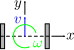
\includegraphics[width=0.25\textwidth]{kinematics.pdf}
	\end{center}
	\caption{The local coordinate frame is centered on the wheel axle, and the forward velocity and angular velocity commands $ v $, $ \omega $ are illustrated as well.}\label{fig:kinematics}
\end{figure}

\section{Velocity Constraints}

The method generates a velocity constraint for each circle in $ C^R $. More precisely, for each robot circle's center point $ P_i^R $, let $ v_x^i $, $ v_y^i $ denote its velocity's coordinates and define a constraint of the form
\begin{align}\label{eq:consRi}
\begin{bmatrix}
n_x^i && n_y^i
\end{bmatrix}
\begin{bmatrix}
v_x^i \\
v_y^i
\end{bmatrix} \leq  b_i ,
\end{align}
which defines an admissible half-plane in the point's velocity space, characterizing it by its boundary's margin $ b_i > 0 $ from the origin and the coordinates $ n_x^i $, $ n_y^i $ of its boundary's outwards unit normal.

The following three sections specify the constraints by defining these parameters as the result of a procedure with three stages. The first stage (Section \ref{sec:vo}) calculates the set of constant relative velocities for the circles $ c_i^{\,R} $ and $ c_i^{\,O} $ that will make them collide within a specific time horizon, which is known as the \textit{relative velocity obstacle}. The second stage (Section \ref{sec:cvo}) calculates a set of admissible relative velocities as a convex approximation of the relative velocity obstacle's complement. The third stage (Section \ref{sec:svo}) shifts the set of admissible relative velocities by the object circle's velocity to obtain the set of admissible velocities for the robot circle.

The final Section \ref{sec:tcvo} describes the transformation to express these constraints as constraints for the velocity of a single reference point $ P^\text{\,ref} $, which is fixed on the robot.

\subsection{Relative Velocity Obstacle}\label{sec:vo}

The set of constant relative velocities that will make two circles collide within a finite time horizon $ \tau $ forms a truncated cone (see Fig. \ref{fig:vo}) and is known as the relative velocity obstacle. The cone's tip represents a frontal collision with a speed of $ D_i/\tau $, where $ D_i = \left|\overrightarrow{P_i^R P_i^O}\right|- r^R - r_i^O - \delta $ includes a small distance margin $ \delta > 0 $. The radius of the truncating arc is equal to $ (r^R + r_i^O)/\tau $. The first stage constructs this set for each object circle and the corresponding robot circle.

\begin{figure}
	\begin{center}
		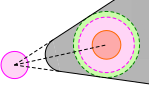
\includegraphics[width=0.75\textwidth]{vo.pdf}
	\end{center}
	\caption{The relative velocity obstacle (grey) for a given time horizon, combining both collider's radii (orange, pink) and an additional margin (green). %Its shape is a truncated cone.
	}\label{fig:vo}
\end{figure}


\subsection{Convex Approximation}\label{sec:cvo}

The second stage is to create a convex approximation of each velocity obstacle's complement to ease subsequent optimization. The method approximates the feasible velocities by a half plane while making it dependent on a given nominal velocity. It is common to maximize in this way the feasible region around the nominal velocity, as this is the region wherein the solution is preferred to be. We also take this approach and compute a tangent halfplane through the velocity obstacle's point which is closest to the nominal velocity if the latter is feasible. In contrast to e.g. ORCA, if the nominal velocity is inside the velocity obstacle, we do not use the boundary point closest to it as the tangent point since it can switch discontinuously from one straight boundary to the other when the nominal velocity crosses the cone's symmetry axis. Instead, we choose as the tangent point the point where the ray from the origin to the nominal velocity intersects the truncating arc. Fig. \ref{fig:cvo_all} shows the resulting continuous half plane generation.

\begin{figure}
	\begin{center}
		\includegraphics[width=\textwidth]{cvo_all_no_borders.pdf}
	\end{center}
	\caption{Top: The mapping from velocities to tangent points to the velocity obstacle boundary. It maps velocities that lie on the same blue line on the same tangent point. Bottom: For different nominal velocities (red arrows), the examples show the corresponding tangent point (blue point) according to this mapping, as well as the resulting half-plane through the tangent point (light grey).}\label{fig:cvo_all}
\end{figure}

\subsection{Shift by Object Velocity}\label{sec:svo}

Assuming that the robot can sense the object circle's velocity, the method shifts the set of admissible relative velocities by the object circle's velocity in order to obtain the set of admissible velocities for the robot circle. However, as the method requires to have a feasible set of constraints since the subsequent optimization must yield a solution, the shift in this stage is limited such that the resulting admissible set contains the origin in order to maintain always the robot's ability to stop.

%\begin{figure}
%	\begin{center}
%		\includegraphics[width=0.75\textwidth]{cvo_1.pdf}
%	\end{center}
%	\caption{.}\label{fig:cvo_1}
%\end{figure}
%
%\begin{figure}
%	\begin{center}
%		\includegraphics[width=0.75\textwidth]{cvo_2.pdf}
%	\end{center}
%	\caption{.}\label{fig:cvo_2}
%\end{figure}
%
%Fig. \ref{fig:cvo_1}
%
%Fig. \ref{fig:cvo_2}

\subsection{Constraints Transformation}\label{sec:tcvo}

The constraints' parameters $ n_x^i$, $ n_y^i $, $ b_i $ result from the geometric constructions described above. To include the constraint for each circle pair $ (c_i^R, c_i^O) $ into a single optimization problem, the method transforms them into constraints for the velocity coordinates $ v_x^\text{ref} $, $ v_y^\text{ref} $ of the single point $ P^\text{\,ref} $ by using the kinematic relations introduced in Section \ref{sec:kinematics}. This transformation is simply
\begin{align}\label{eq:consVref}
\begin{bmatrix}
n_x^i && n_y^i
\end{bmatrix}
J_{P_i^R} J_{P^\text{\,ref}}^{-1}
\begin{bmatrix}
v_x^\text{ref} \\
v_y^\text{ref}
\end{bmatrix} \leq  b_i .
\end{align}

\section{Constrained Optimization}

The method computes the velocity command tuple $ (v^*,  \omega^* ) $ which the robot will execute by minimizing its deviation from a given nominal command $ (\bar v, \bar\omega) $ coming from the driver or any higher-level module. It achieves collision avoidance by imposing the constraints \eqref{eq:consVref} on this optimization. This minimization is performed directly in the space of the reference point velocity, i.e. over $ v_x^\text{ref} $, $ v_y^\text{ref} $. Therefore, we transform the nominal command into a corresponding nominal velocity for the reference point $ {\left[ \bar v_x^\text{ref}, \bar v_y^\text{ref} \right]}^T = J_{P^\text{\,ref}} {\left[ \bar v, \bar\omega  \right]}^T$. The optimization problem is formally written as
\begin{equation}\label{eq:qp}
\begin{aligned}
(v_x^{\text{ref}*}, v_y^{\text{ref}*}) = & \arg\min_{v_x^\text{ref}, v_y^\text{ref}}~ (v_x^\text{ref} - \bar v_x^\text{ref})^2 + (v_y^\text{ref} - \bar v_y^\text{ref})^2 \\
\text{s.t. } & \begin{bmatrix}
n_x^i && n_y^i
\end{bmatrix}
J_{P_i^R} J_{P^\text{\,ref}}^{-1}
\begin{bmatrix}
v_x^\text{ref} \\
v_y^\text{ref}
\end{bmatrix} \leq  b_i, ~\forall i \in {1, ..., N}.
\end{aligned}
\end{equation}
From the solution, the actual velocity command for the robot is then computed as $ {\left[ v^*, \omega^*  \right]}^T = J_{P^\text{\,ref}}^{-1} {\left[ v_x^{\text{ref}*}, v_y^{\text{ref}*} \right]}^T $.

The constraints \eqref{eq:consVref} are feasible by construction, as they always keep the origin free, i.e. the robot is always allowed to stop. Hence, the optimization problem \eqref{eq:qp} always has a solution.

\appendix

\section{Kinematics}\label{app:kinematics}

Let the coordinates $ x^P, y^P $ and $ v_x^P, v_y^P $ describe respectively the position (relative to the local frame's center) and the velocity (i.e. the derivative of the position relative to a static point) of a point $ P $ on the robot when expressed in the local coordinate frame (shown in Fig. \ref{fig:kinematics}). It holds for any point $ P $ on the robot that
\begin{align}\label{eq:J}
\begin{bmatrix}
v_x^P \\
v_y^P
\end{bmatrix}
= 
J_P
\begin{bmatrix}
v \\
\omega
\end{bmatrix} = 
\begin{bmatrix}
0 && - y^P\\
1 && x^P
\end{bmatrix}
\begin{bmatrix}
v \\
\omega
\end{bmatrix} .
\end{align}
Any point $ P $'s velocity vector is sufficient to determine $ v $ and $ \omega $ if $ P $ does not have a vanishing $ y^P $ and thus \eqref{eq:J} is invertible. Then, the inverse is given by
\begin{align}\label{eq:J^-1}
\begin{bmatrix}
v \\
\omega
\end{bmatrix}
=
J_P^{-1}
\begin{bmatrix}
v_x^P \\
v_y^P
\end{bmatrix} =
\begin{bmatrix}
x^P/y^P && 1\\
-1/y^P && 0
\end{bmatrix}
\begin{bmatrix}
v_x^P \\
v_y^P
\end{bmatrix} .
\end{align}

Choose two different points $ P $ and $ P' $ and chain the relation \eqref{eq:J} for $ P' $ with the relation \eqref{eq:J^-1} for $ P $ by replacing $ v $, $ \omega $ to obtain
\begin{align}\label{eq:Jpp}
\begin{bmatrix}
v_x^{P'} \\
v_y^{P'}
\end{bmatrix}
= 
J_{P'}J_P^{-1}
\begin{bmatrix}
v_x^P \\
v_y^P
\end{bmatrix} = 
\begin{bmatrix}
y^{P'}/y^P && 0\\
(x^P - x^{P'})/y^P && 1
\end{bmatrix}
\begin{bmatrix}
v_x^P \\
v_y^P
\end{bmatrix} .
\end{align}
This relation maps the velocity of any point $ P $ which does not lie on the x-axis to any other point's velocity. Denoting the matrix from \eqref{eq:Jpp} by $ M =  J_{P'}J_P^{-1}$, one calculates
\begin{align*}
M^TM = \begin{bmatrix}
{\left(y^{P'}/y^P\right)}^2 + {\left((x^P - x^{P'})/y^P\right)}^2 && (x^P - x^{P'})/y^P\\
(x^P - x^{P'})/y^P && 1
\end{bmatrix} .
\end{align*}
The eigenvalues $ \lambda_{1,2} $ of $ M^TM $ follow as
\begin{align*}
\lambda_{1,2} = \cfrac{y_P^2 + y_{P'}^2 + {\left(x_P - x_{P'}\right)}^2 \pm \sqrt{{\left(y_P^2 + y_{P'}^2 + {\left(x_P - x_{P'}\right)}^2\right)}^2 - 4y_P^2y_{P'}^2}}{2y_P^2} .
\end{align*}
For the case that $ x^P = x^{P'} $, the larger eigenvalue is given by
\begin{align*}
\lambda_\text{max} = \begin{cases}1\quad\quad&y_{P'}^2 \leq y_P^2\\\cfrac{y_{P'}^2}{y_P^2}\quad\quad &y_{P'}^2 > y_P^2\end{cases}.
\end{align*}

\end{document}